Los resultados obtenidos se presentan a continuación mediante gráficos generados automáticamente a partir de los datos producidos por los algoritmos.

\subsection*{Tiempo de ejecución}

La Figura~\ref{fig:tiempo_bf_greedy} muestra el tiempo de ejecución de fuerza bruta y los dos greedy. Se observa que greedy1 crece linealmente con $n$, llegando a aproximadamente 60 µs para $n=200$, mientras que greedy2 es consistentemente más rápido, llegando a 21 µs. Fuerza bruta solo aparece para $n \in \{3,5,8\}$ y su tiempo es irregular dado que depende fuertemente de los valores aleatorios de $M$ y $E$.

\begin{figure}[H]
    \centering
    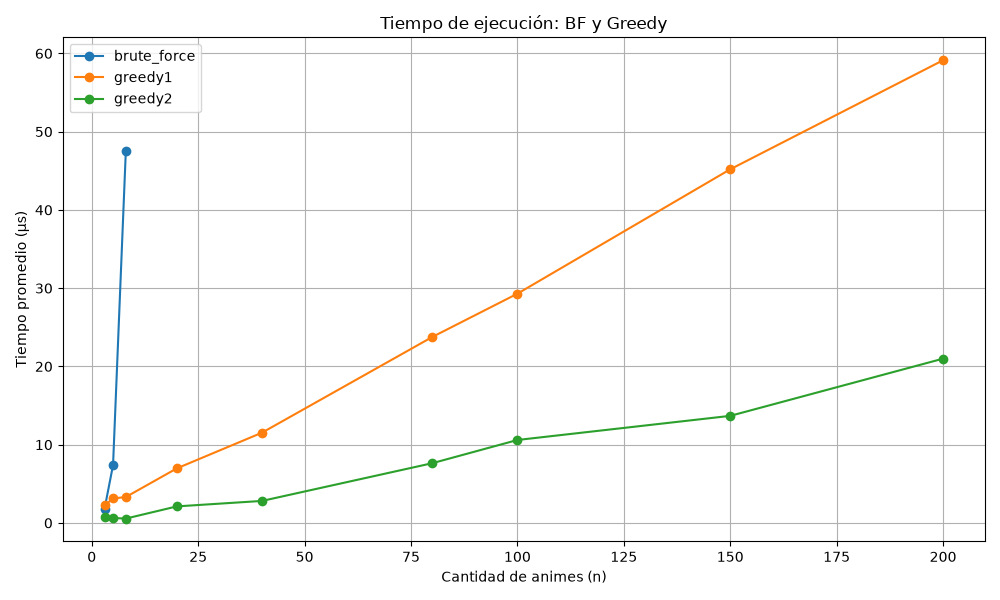
\includegraphics[width=0.85\textwidth]{../code/implementation/data/plots/tiempo_bf_greedy.png}
    \caption{Tiempo de ejecución de Fuerza Bruta y Greedy según cantidad de animes.}
    \label{fig:tiempo_bf_greedy}
\end{figure}

La Figura~\ref{fig:tiempo_dp} muestra el tiempo de DP de forma separada dada la diferencia de escala. Se aprecia una tendencia creciente general, aunque con variaciones producto de los valores aleatorios de $M$ y $E$ en cada caso, ya que la complejidad de DP es $O(n \cdot q \cdot M \cdot E)$ y los tres últimos factores varían entre instancias.

\begin{figure}[H]
    \centering
    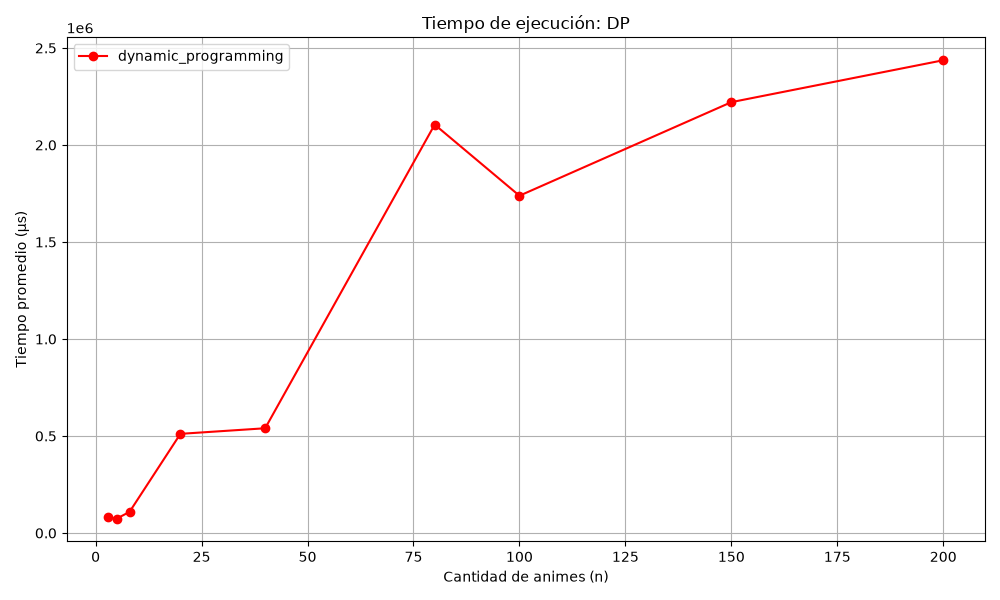
\includegraphics[width=0.85\textwidth]{../code/implementation/data/plots/tiempo_dp.png}
    \caption{Tiempo de ejecución de Programación Dinámica según cantidad de animes.}
    \label{fig:tiempo_dp}
\end{figure}

\subsection*{Uso de memoria}

La Figura~\ref{fig:memoria} muestra el uso de memoria de cada algoritmo. DP utiliza aproximadamente 16.000 KB de forma constante independiente de $n$, lo cual se explica porque la tabla \texttt{dp[3001][501]} se declara globalmente con tamaño fijo máximo ($3001 \times 501 \times 8$ bytes $\approx$ 12 MB), sin importar el tamaño real de la instancia. Los demás algoritmos mantienen un uso constante de aproximadamente 4.000 KB correspondiente a la memoria base del proceso.

\begin{figure}[H]
    \centering
    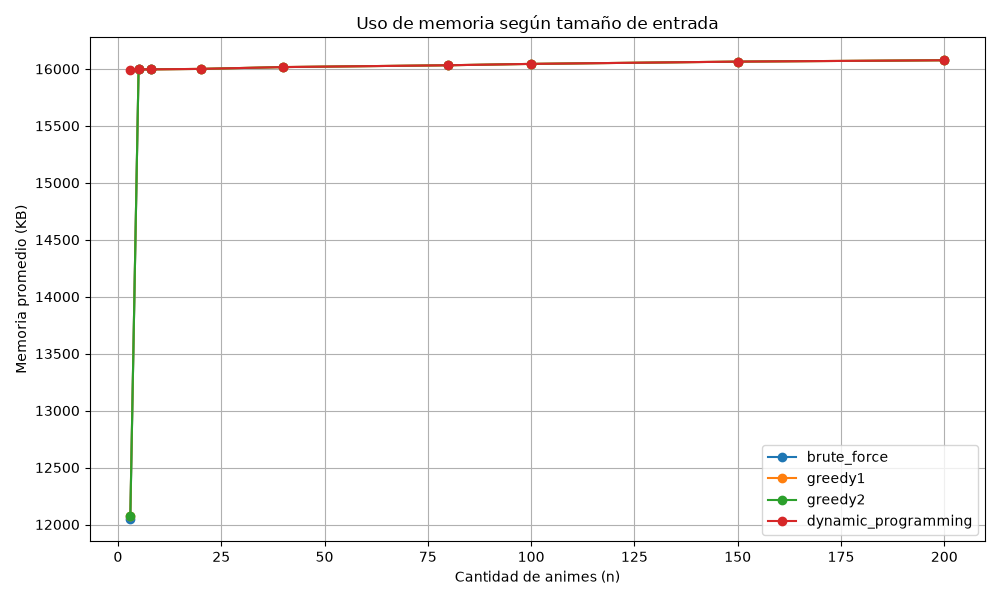
\includegraphics[width=0.85\textwidth]{../code/implementation/data/plots/memoria.png}
    \caption{Uso de memoria según cantidad de animes.}
    \label{fig:memoria}
\end{figure}

\subsection*{Calidad de solución}

Las Figuras~\ref{fig:calidad_g1} y \ref{fig:calidad_g2} muestran el porcentaje del óptimo alcanzado por cada greedy respecto a DP. Greedy1, que ordena por bono de completación, alcanza entre un 22\% y 78\% del óptimo, con tendencia a empeorar para instancias grandes. Esto se debe a que ignorar el costo en tiempo y energía al priorizar por bono es una decisión local que no refleja bien el valor real de cada anime. Greedy2, que usa el criterio $v/(t+c)$, se desempeña considerablemente mejor, alcanzando entre un 61\% y 98\% del óptimo, lo que confirma que considerar el costo de los recursos mejora significativamente la calidad de la solución.

\begin{figure}[H]
    \centering
    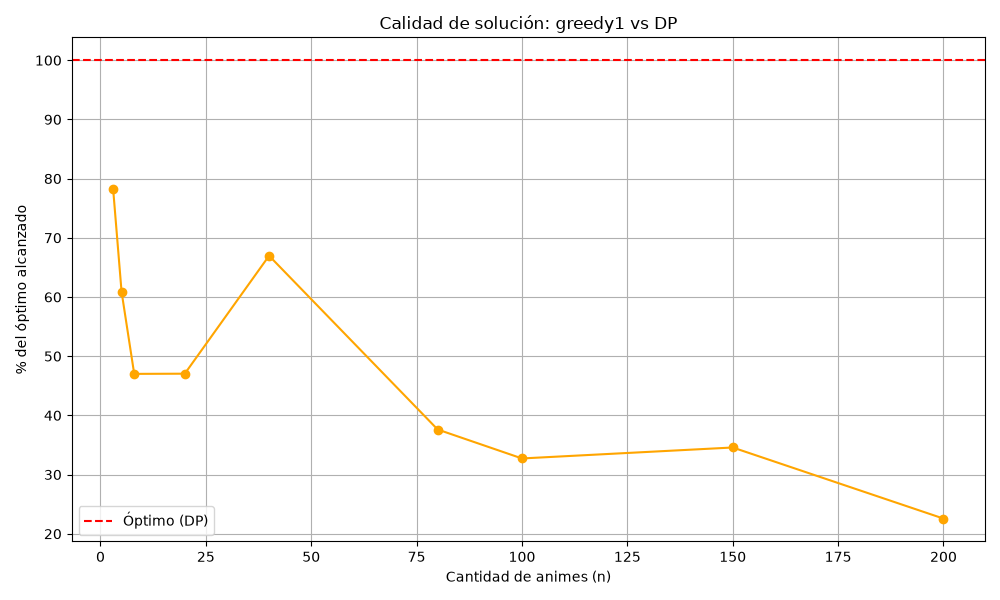
\includegraphics[width=0.85\textwidth]{../code/implementation/data/plots/calidad_greedy1.png}
    \caption{Porcentaje del óptimo alcanzado por Greedy1 respecto a DP.}
    \label{fig:calidad_g1}
\end{figure}

\begin{figure}[H]
    \centering
    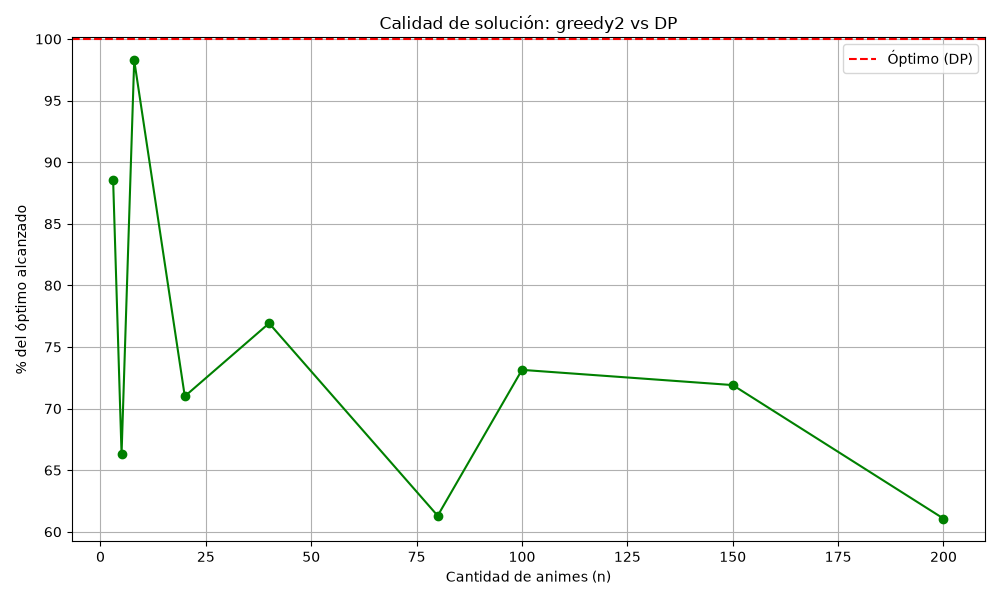
\includegraphics[width=0.85\textwidth]{../code/implementation/data/plots/calidad_greedy2.png}
    \caption{Porcentaje del óptimo alcanzado por Greedy2 respecto a DP.}
    \label{fig:calidad_g2}
\end{figure}

\subsection*{Comportamiento al variar parámetros}

Las Figuras~\ref{fig:ctrl_n}, \ref{fig:ctrl_M}, \ref{fig:ctrl_E} y \ref{fig:ctrl_q} muestran el tiempo de ejecución variando cada parámetro de forma controlada. En todos los casos, greedy1 y greedy2 permanecen prácticamente en 0 µs, confirmando su independencia de estos parámetros. DP en cambio crece linealmente al aumentar $n$, $M$, $E$ y $q$, lo cual es consistente con su complejidad teórica $O(n \cdot q \cdot M \cdot E)$.

\begin{figure}[H]
    \centering
    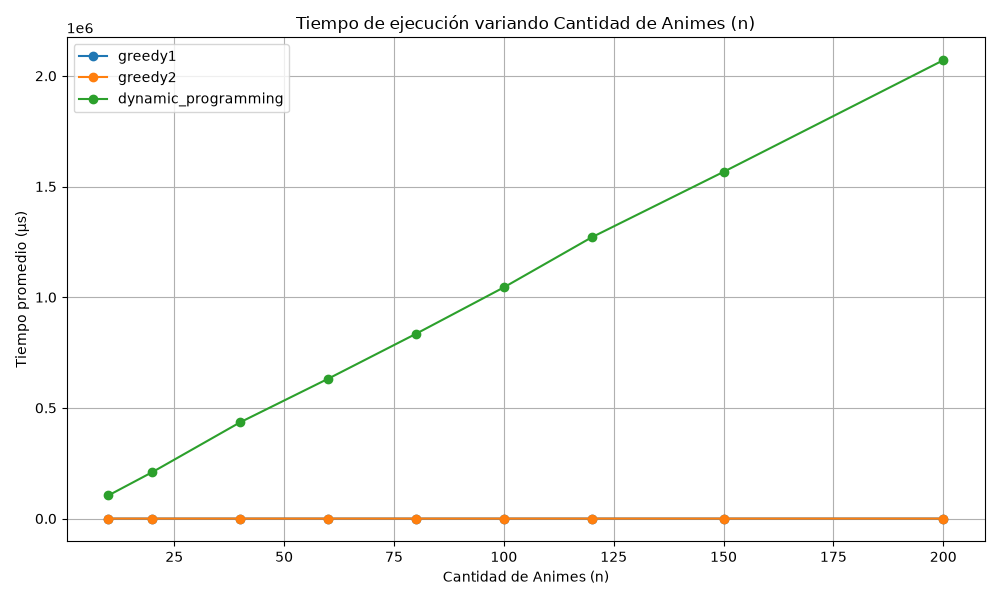
\includegraphics[width=0.85\textwidth]{../code/implementation/data/plots/control_tiempo_n.png}
    \caption{Tiempo de ejecución variando cantidad de animes $n$ (M=1500, E=250 fijos).}
    \label{fig:ctrl_n}
\end{figure}

\begin{figure}[H]
    \centering
    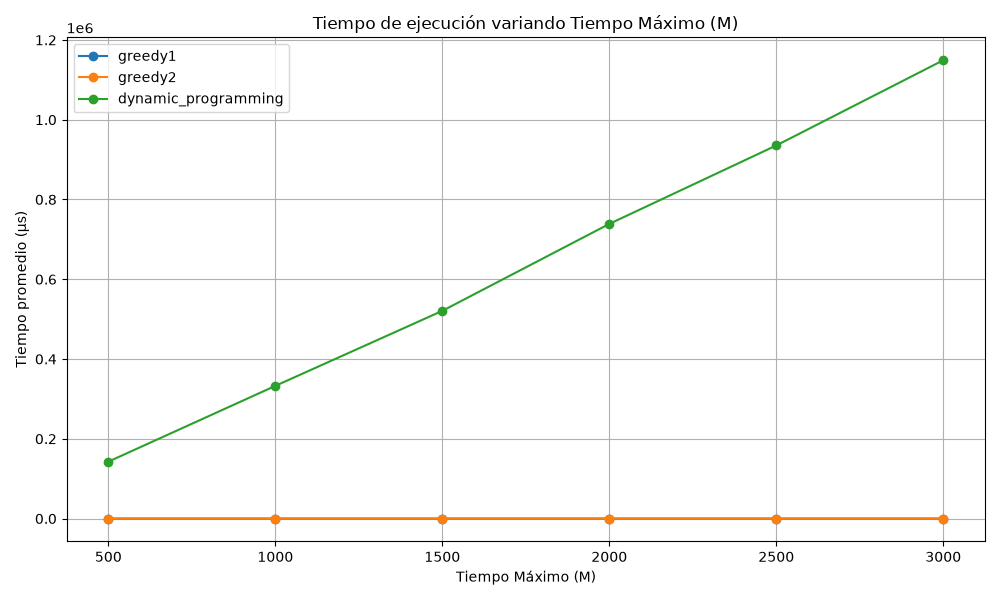
\includegraphics[width=0.85\textwidth]{../code/implementation/data/plots/control_tiempo_M.png}
    \caption{Tiempo de ejecución variando minutos disponibles $M$ (n=50, E=250 fijos).}
    \label{fig:ctrl_M}
\end{figure}

\begin{figure}[H]
    \centering
    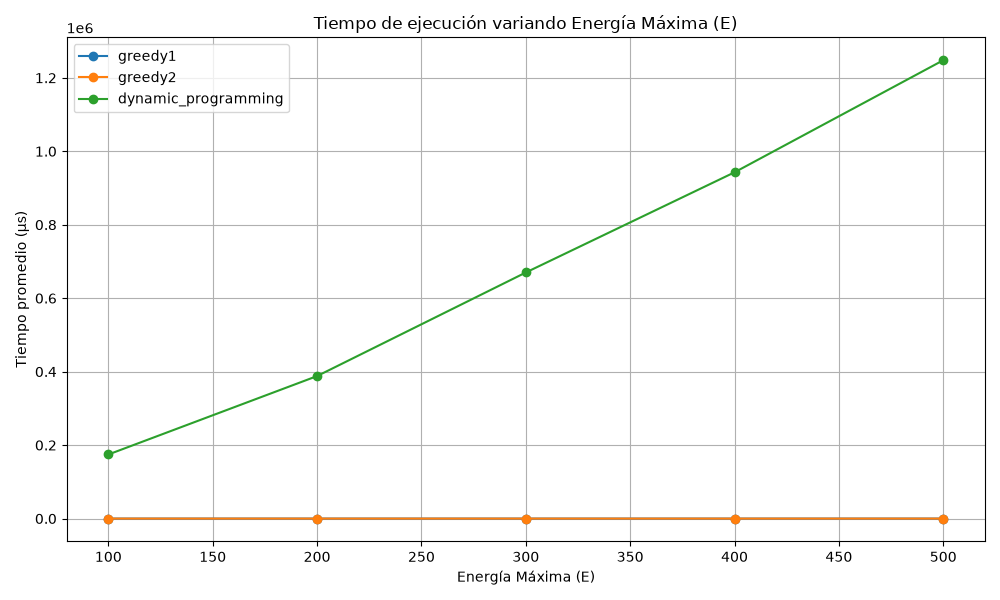
\includegraphics[width=0.85\textwidth]{../code/implementation/data/plots/control_tiempo_E.png}
    \caption{Tiempo de ejecución variando energía disponible $E$ (n=50, M=1500 fijos).}
    \label{fig:ctrl_E}
\end{figure}

\begin{figure}[H]
    \centering
    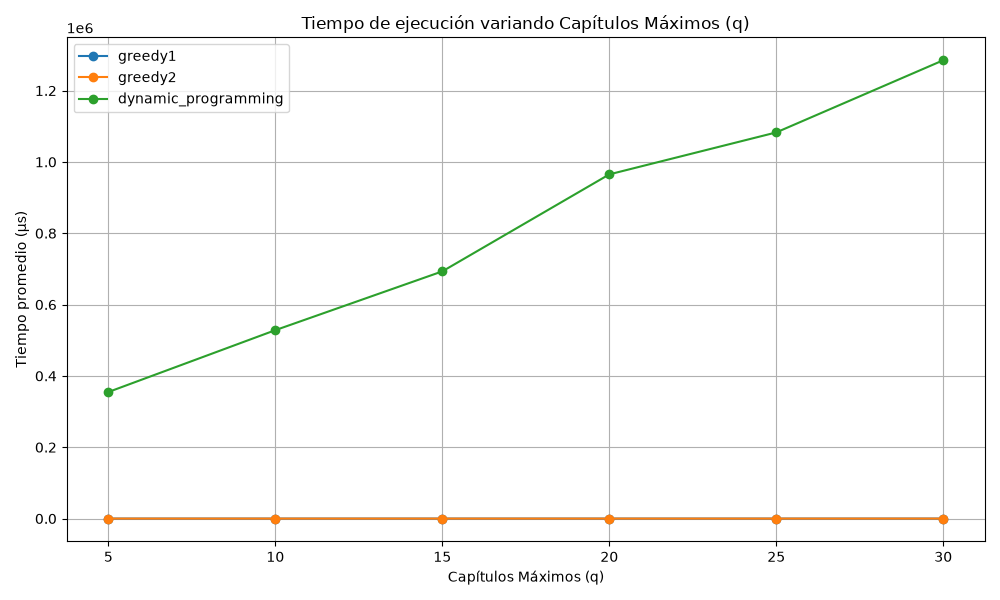
\includegraphics[width=0.85\textwidth]{../code/implementation/data/plots/control_tiempo_q.png}
    \caption{Tiempo de ejecución variando capítulos máximos $q$ (n=50, M=1500, E=250 fijos).}
    \label{fig:ctrl_q}
\end{figure}